\documentclass{beamer}
%\mode<presentation>
\usepackage[utf8]{inputenc}
\usepackage[english]{babel}
\usetheme{CambridgeUS}
\usecolortheme{dolphin}
\usepackage{amsmath,amssymb,amsfonts, bm}
\usepackage{mathpazo}
\usepackage{graphicx,tabularx,epsfig}
\usepackage[compatibility=false]{caption}
\usepackage{subcaption}
\usepackage{rotating}
\usepackage{mathtools}


\setbeamertemplate{background}{\tikz[overlay,remember picture]\node[opacity=0.07]at (current page.center){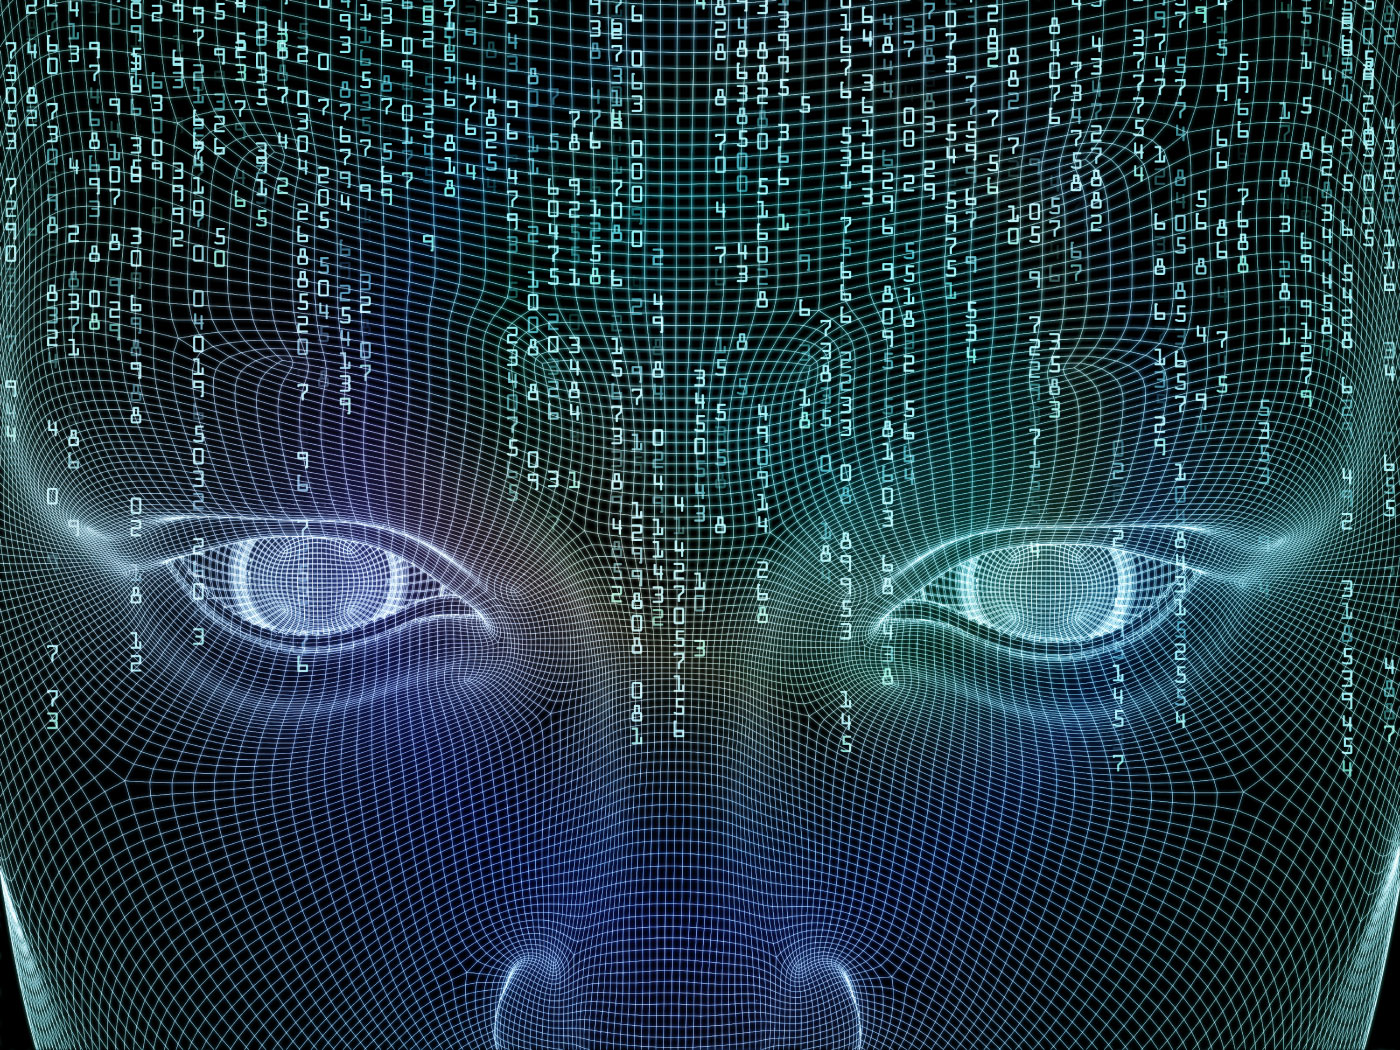
\includegraphics[width=\paperwidth]{pic/bkg}};}
\usepackage{tikz}

\DeclareGraphicsExtensions{.pdf,.png,.jpg,.svg}


\setbeamertemplate{itemize items}[square]
\setbeamertemplate{enumerate items}[square]

\definecolor{Red}{RGB}{190,0,0}
\definecolor{Blue}{RGB}{0,0,190}
\setbeamertemplate{headline}{}



\title[Three particle Levy HBT]{\Large{PHENIX PLHF PWG}\\Three particle Bose-Einstein correlation}
\author[Attila Bagoly]{Attila Bagoly\\ Eötvös Loránd University \vspace{0.5cm}}
\date[\today]{\today}
\institute[ELTE]{
\large{Supervisor: Máté Csanád}
}

\begin{document}

\begin{frame}
  \titlepage
\end{frame}


\section{What and how we measure}
\begin{frame}
\frametitle{Details of measurement}
\begin{itemize}
\setlength{\itemsep}{22pt}
\item PPG194 generalized to three particle
\item Event-mixing method to measure correlation
\item Momentum difference distributions of pion pairs within the triplet from same event: $A(k_{12}, k_{13}, k_{23})$
\item Background distribution (triplets from different events): $B(k_{12}, k_{13}, k_{23})$
\item Same global, track and pair cuts as PPG194
\end{itemize}
\end{frame}

\begin{frame}
\frametitle{Three-particle Bose-Einstein correlation function}
\begin{itemize}
\setlength{\itemsep}{18pt}
\item Correlation function:
\begin{equation}
C_3(\bm{k_1}, \bm{k_2}, \bm{k_3})=\frac{N_3(\bm{k_1}, \bm{k_2}, \bm{k_3})}{N_1(\bm{k_1})N_1(\bm{k_2})N_1(\bm{k_3})}
\end{equation}
\item Three particle momentum distribution:
\end{itemize}
\begin{equation}
N(\bm{k_1}, \bm{k_2}, \bm{k_3}) = \int S(\bm{r_1}, \bm{k_1})S(\bm{r_2}, \bm{k_2})S(\bm{r_3}, \bm{k_3})|\Psi_{\bm{k_1, k_2, k_3}}(\bm{r_1},\bm{r_2},\bm{r_3})|^2 \Pi_{i=0}^{3} d^4 \bm{r_i}
\end{equation}
\begin{itemize}
\setlength{\itemsep}{18pt}
\item Assumption for source: Levy-distribution

\item Coulomb-correction:
\begin{equation}
C_3(\bm{k_1}, \bm{k_2}, \bm{k_3}) = C_3^{(0)}(\bm{k_1}, \bm{k_2}, \bm{k_3})K(\bm{k_1}, \bm{k_2}, \bm{k_3})
\end{equation}
\item Coulomb-correction from Generalized Riverside
\item Coulomb-correction parameters obtained from PPG194
\end{itemize}
\end{frame}


\begin{frame}
\frametitle{Quantum statistical correlation function}
\begin{itemize}
\setlength{\itemsep}{16pt}
\item Dimension: 9D $\rightarrow$ 3D
\item Approximation for $C_3^{(0)}$ can be derived (similar as in PPG194):
\begin{align}
C_3^{(0)}(k_{12}, k_{13}, k_{23}) = 1+ \ell_3e^{-0.5(|2k_{12}R|^\alpha+|2k_{13}R|^\alpha+|2k_{23}R|^\alpha)}\nonumber\\
+\ell_2\bigg(e^{|2k_{12}R|^\alpha}+e^{|2k_{13}R|^\alpha}+e^{|2k_{23}R|^\alpha}\bigg)
\end{align}
\item Background: $N(1+\epsilon k_{12})(1+\epsilon k_{13})(1+\epsilon k_{23})$
\item Fitted parameters: $\ell_2, \ell_3$, $\epsilon$, $N$
\item We already know (from PPG194): $R$, $\alpha$
\item We are looking for: $\lambda_3=\ell_3+3\ell_2$
\end{itemize}
\end{frame}


\section{Fittings}

\begin{frame}
\frametitle{Diagonal visualization of fits}
\begin{itemize}
\setlength{\itemsep}{10pt}
\item Visualization in $k_{12}=k_{13}=k_{23}$ subspace:  shows good fits
\item Fitted: $\ell_2$, $\ell_3$, $\epsilon$, $N$; Fixed (PPG194): $R$, $\alpha$
\end{itemize}
\begin{figure}
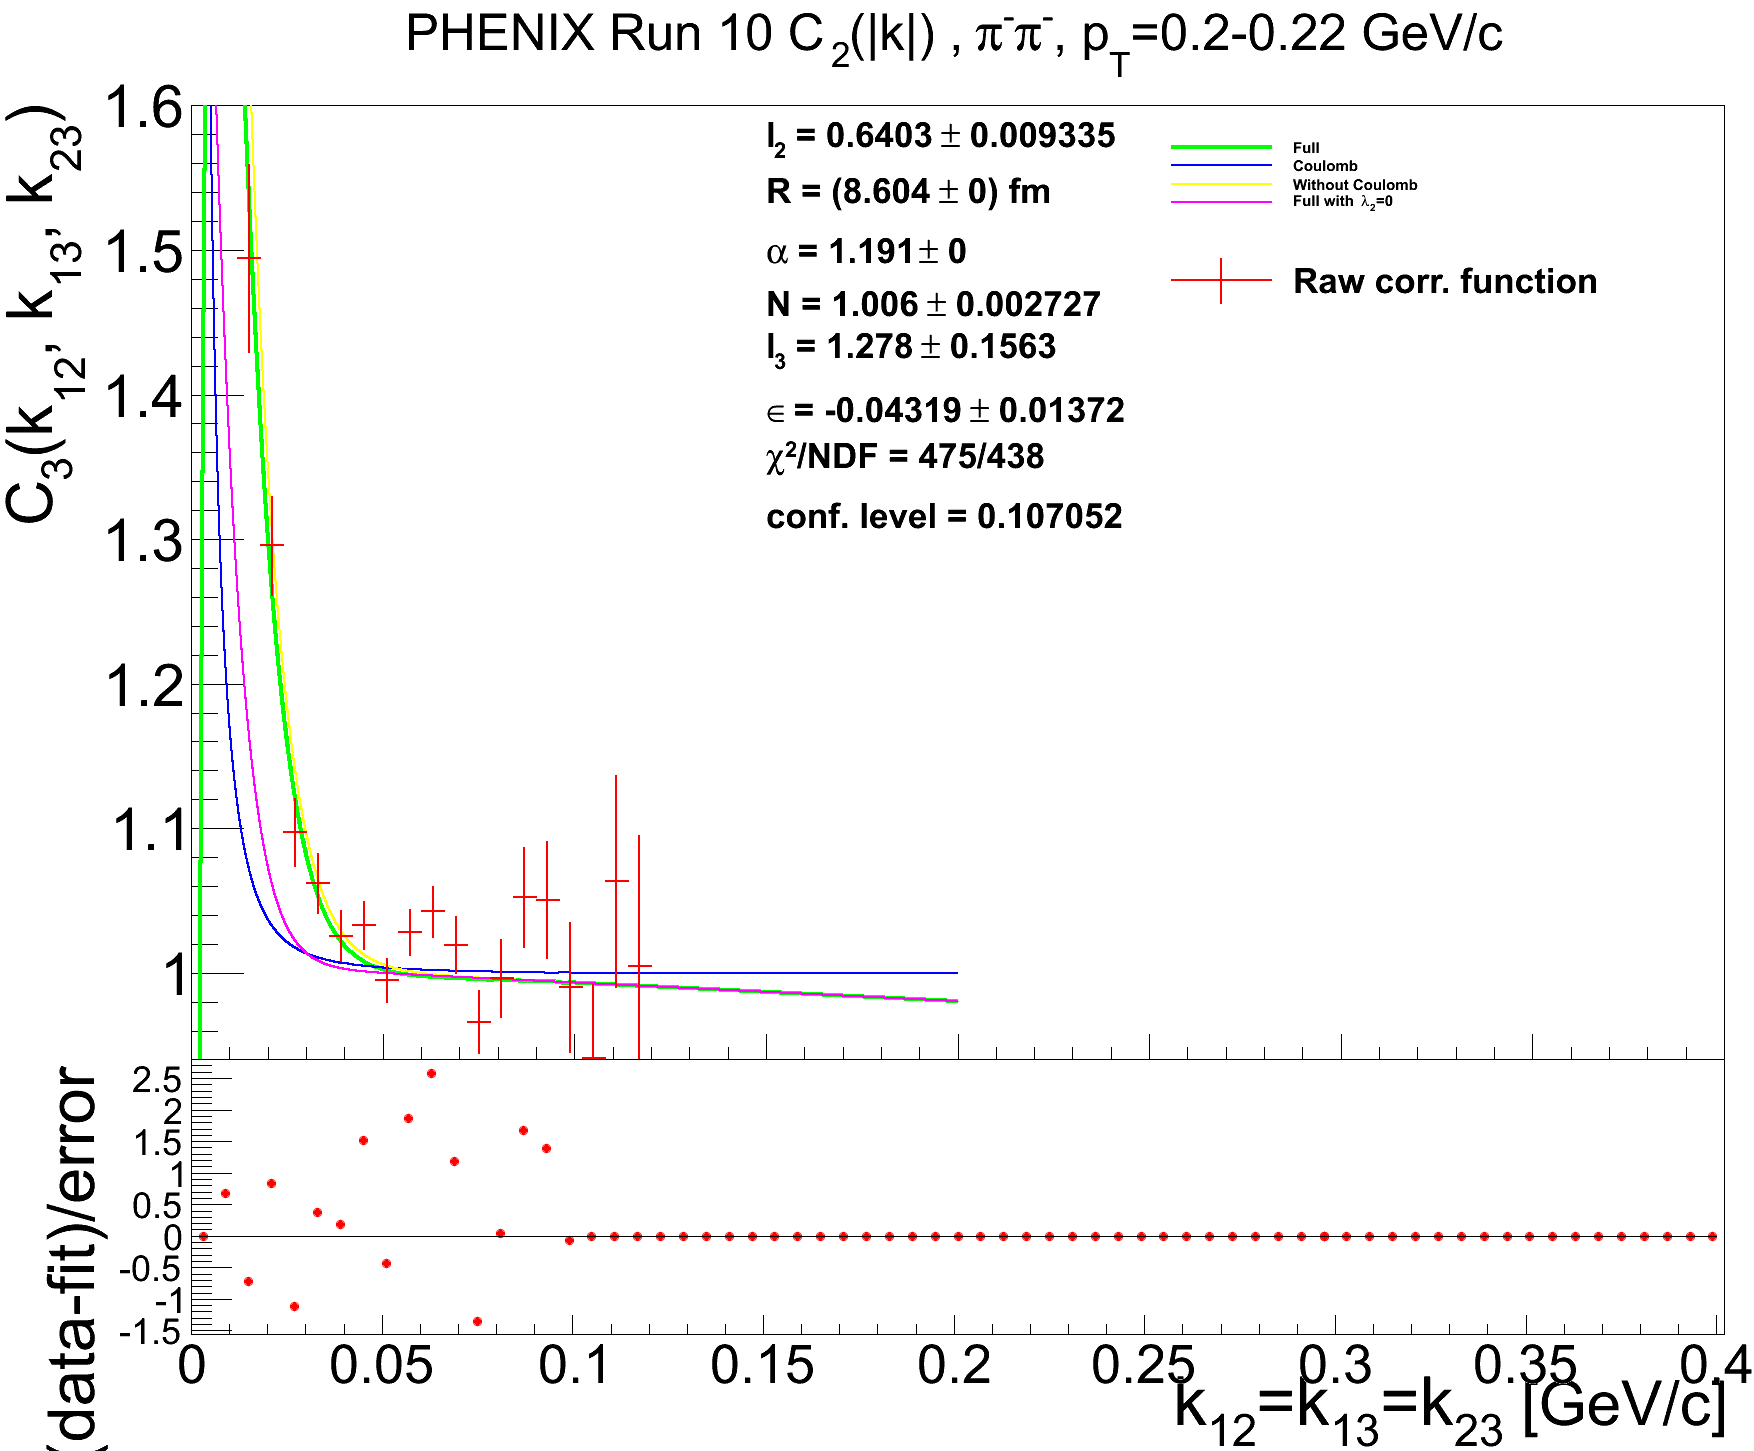
\includegraphics[scale=0.13]{pic/C_icharge0_pt2}
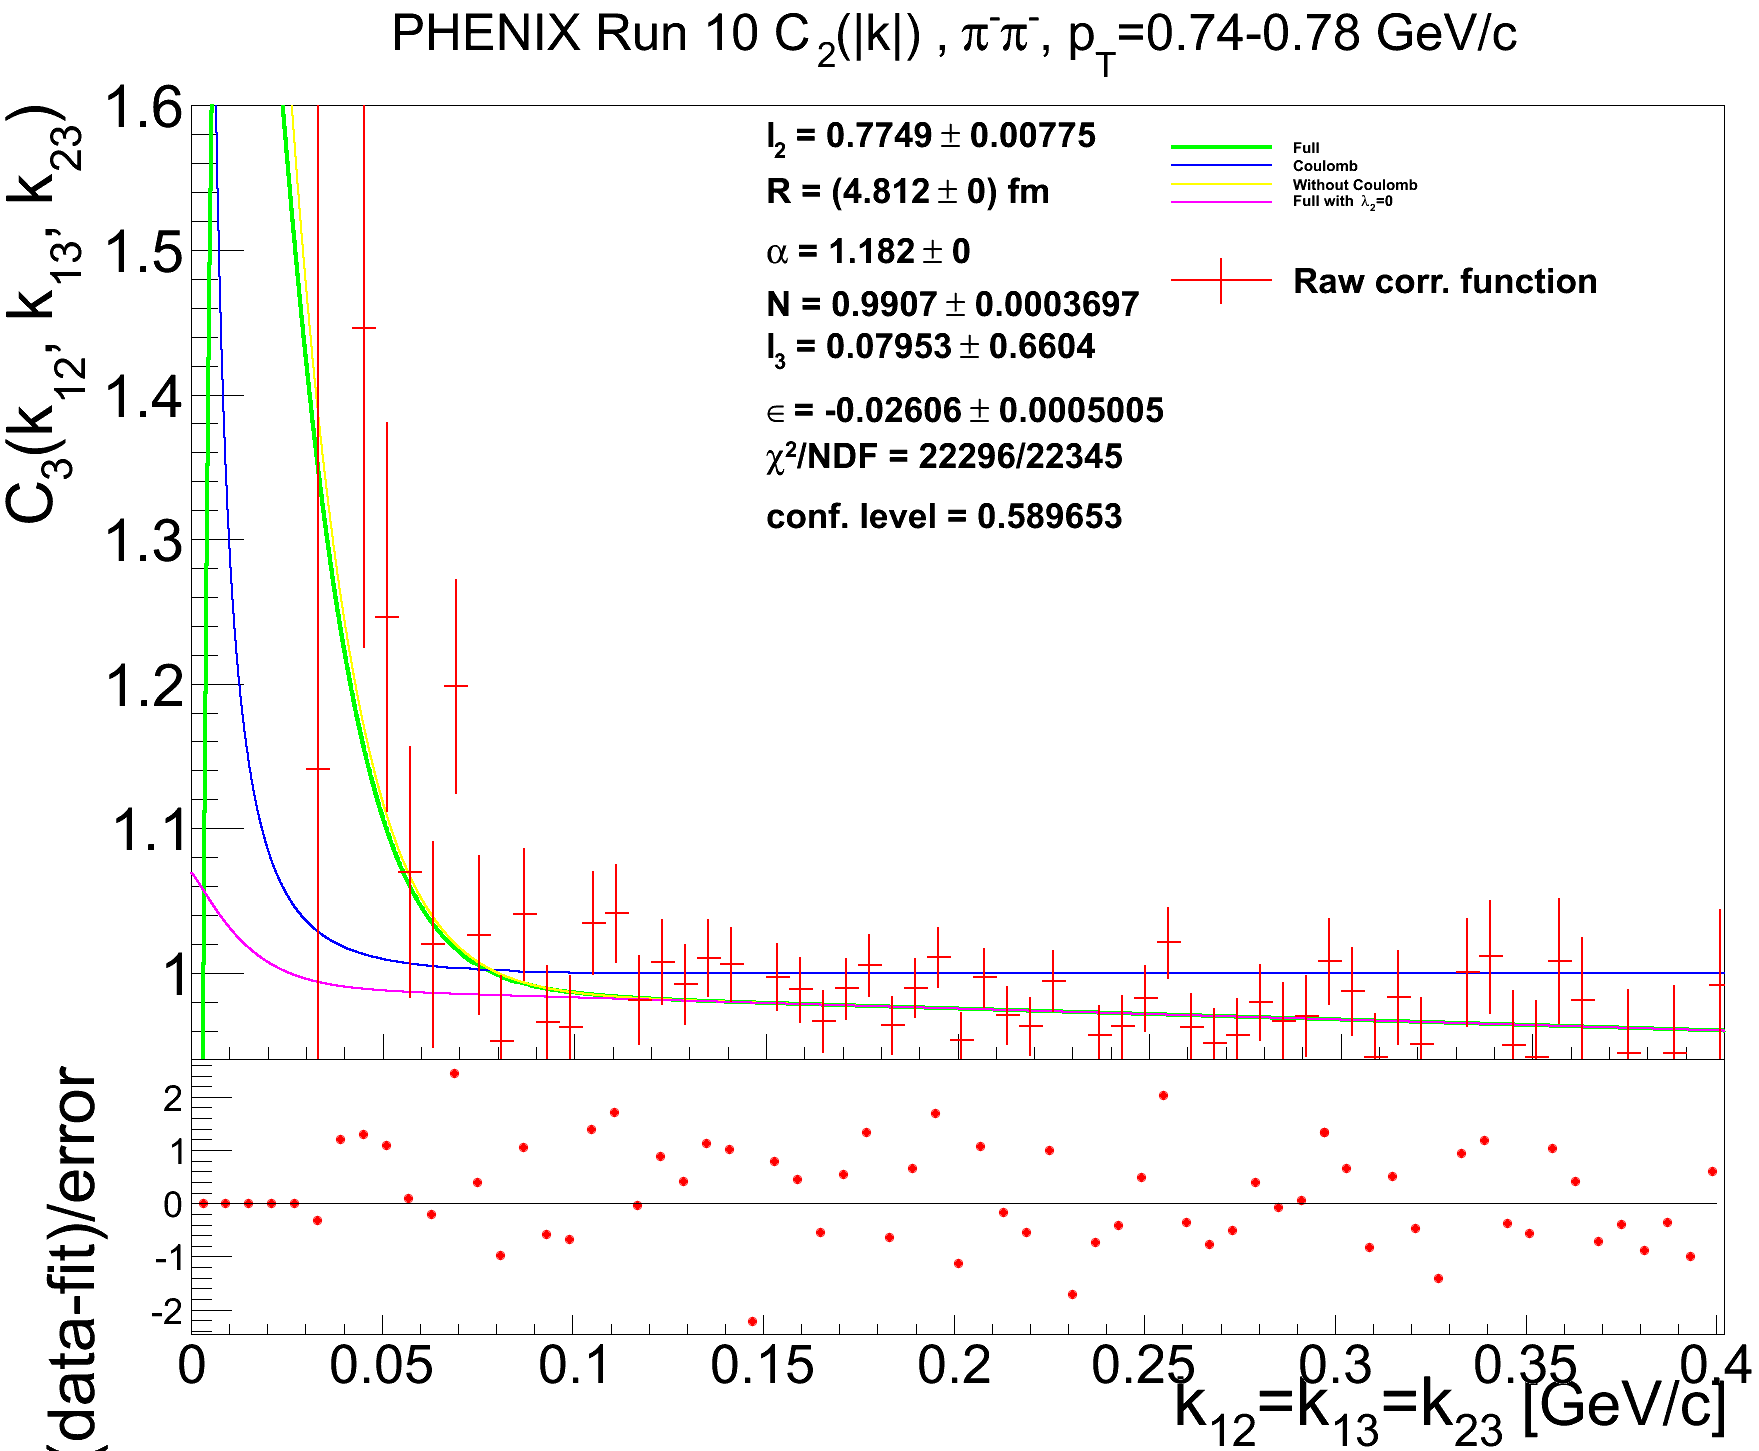
\includegraphics[scale=0.13]{pic/C_icharge0_pt29}

\end{figure}
\end{frame}


\begin{frame}
\frametitle{$\chi^2/NDF$}
\begin{itemize}
\setlength{\itemsep}{10pt}
\item $p_T$ divided into 32 bins
\item Fitted: $\ell_2$, $\ell_3$, $\epsilon$, $N$; Fixed (PPG194): $R$, $\alpha$
\item Quite good $\chi^2/NDF$, not so good confidence levels for mid $p_T$
\end{itemize}
\begin{figure}
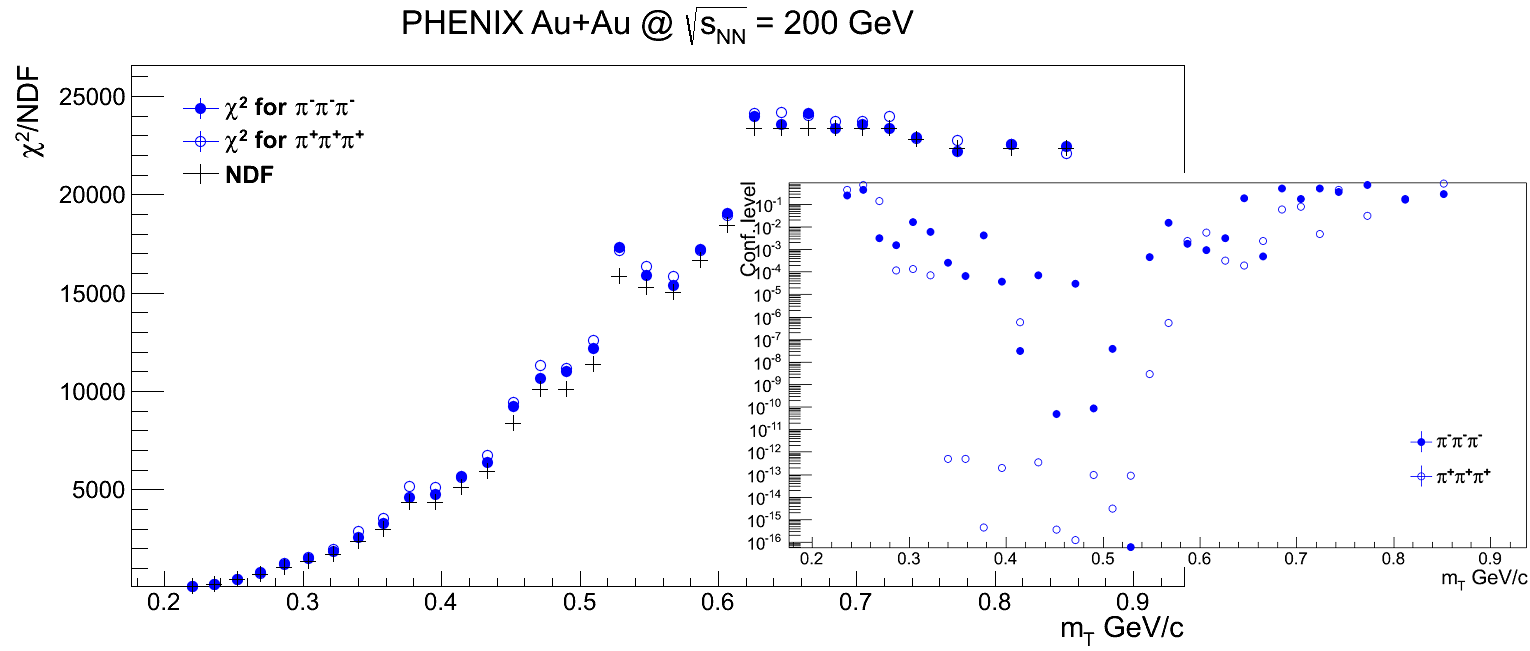
\includegraphics[scale=0.38]{pic/chi2confl}
%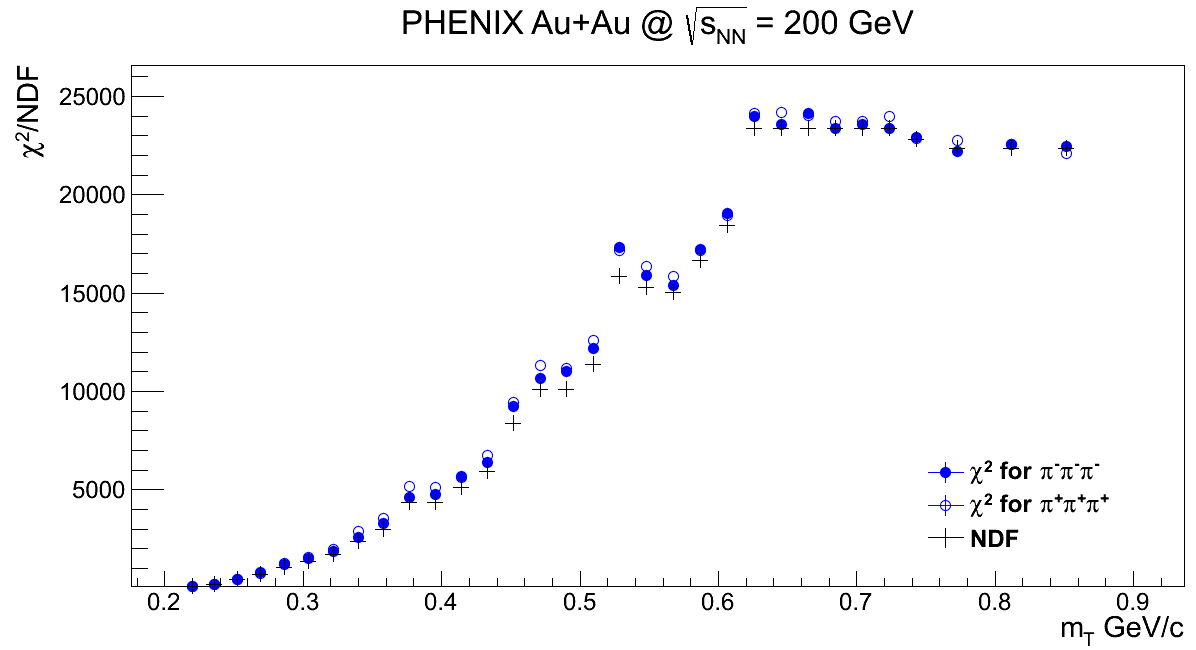
\includegraphics[scale=0.25]{pic/chi2}
%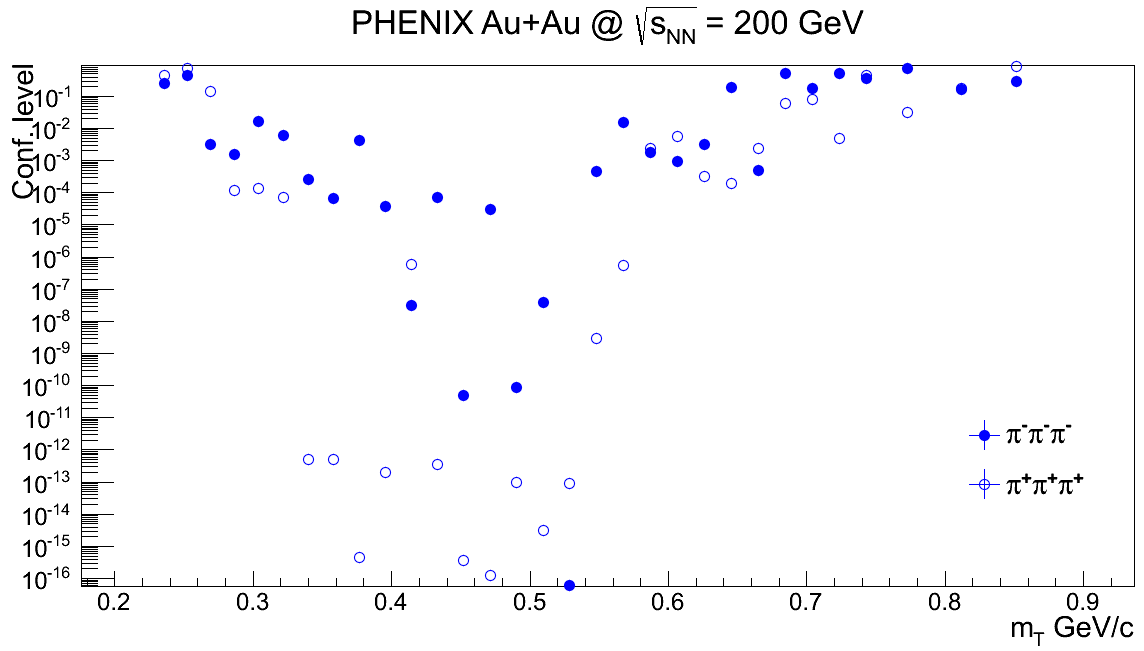
\includegraphics[scale=0.15]{pic/confl}
\end{figure}
\end{frame}



\begin{frame}
\frametitle{Fit parameter $\epsilon$ and $N$}
\begin{itemize}
\setlength{\itemsep}{10pt}
\item Fitted: $\ell_2$, $\ell_3$, $\epsilon$, $N$, Fixed (PPG194): $R$, $\alpha$
\item $N$, $\epsilon$ looks like in PPG194
\end{itemize}
\begin{figure}
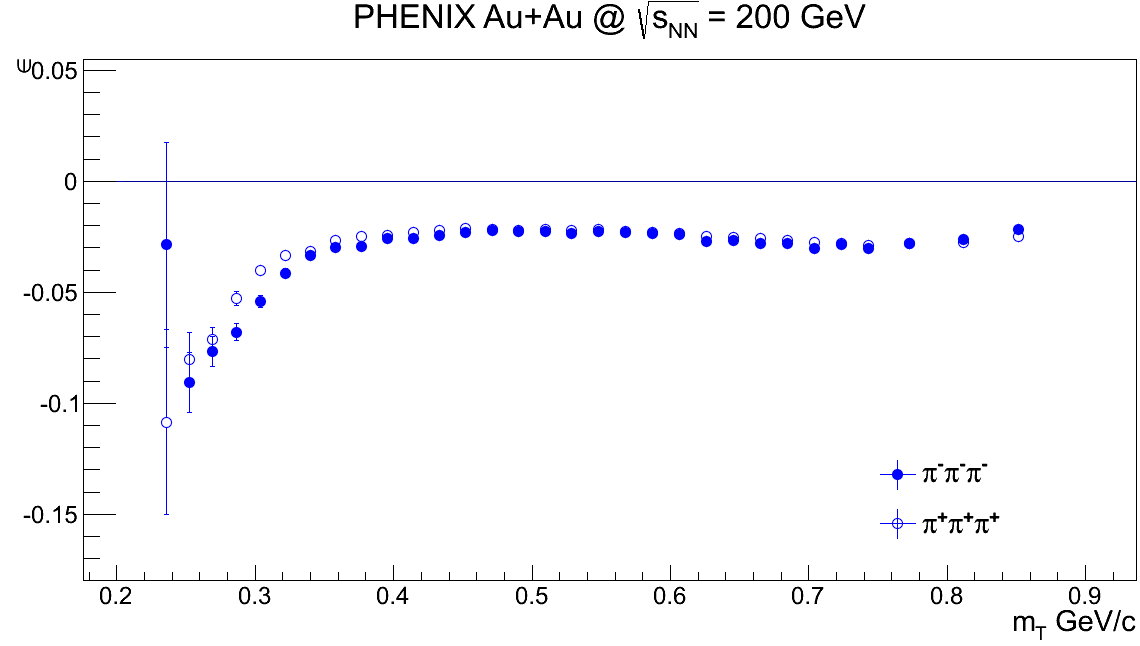
\includegraphics[scale=0.2]{pic/epsilon}
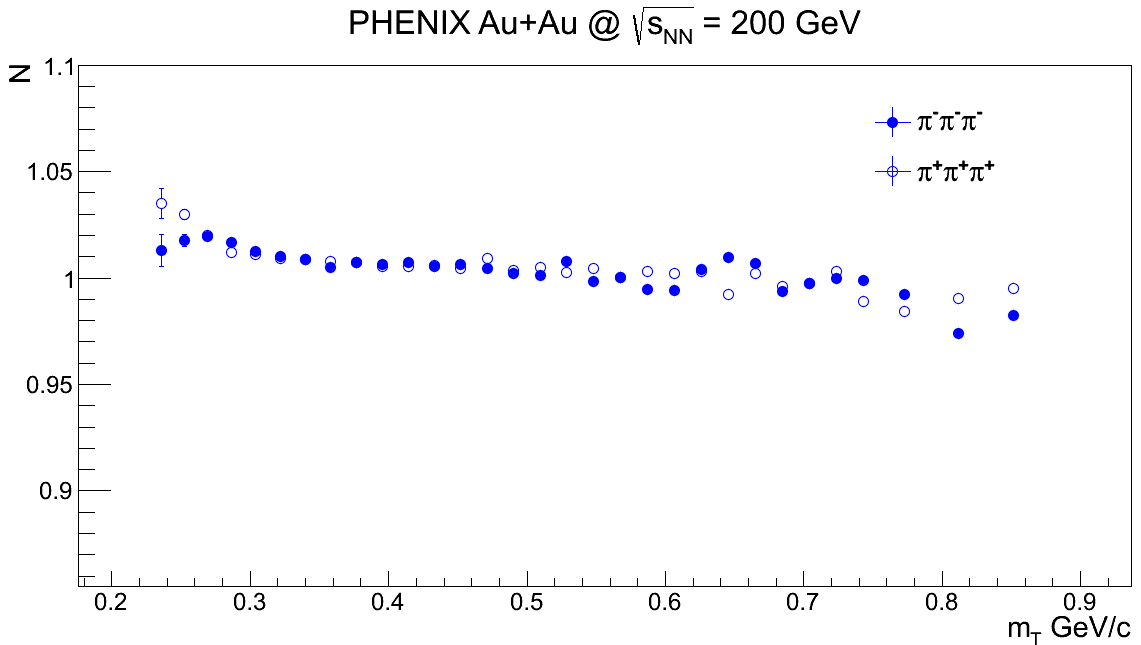
\includegraphics[scale=0.2]{pic/N}

\end{figure}
\end{frame}

\begin{frame}
\frametitle{Fit parameter $\ell_2$ and $\ell_3$}
\begin{itemize}
\setlength{\itemsep}{10pt}
\item Fitted: $\ell_2$, $\ell_3$, $\epsilon$, $N$; Fixed (PPG194): $R$, $\alpha$
\item fitting with small error for $\ell_2$
\item bigger error for $\ell_3$ at high $p_T$
\end{itemize}
\begin{figure}
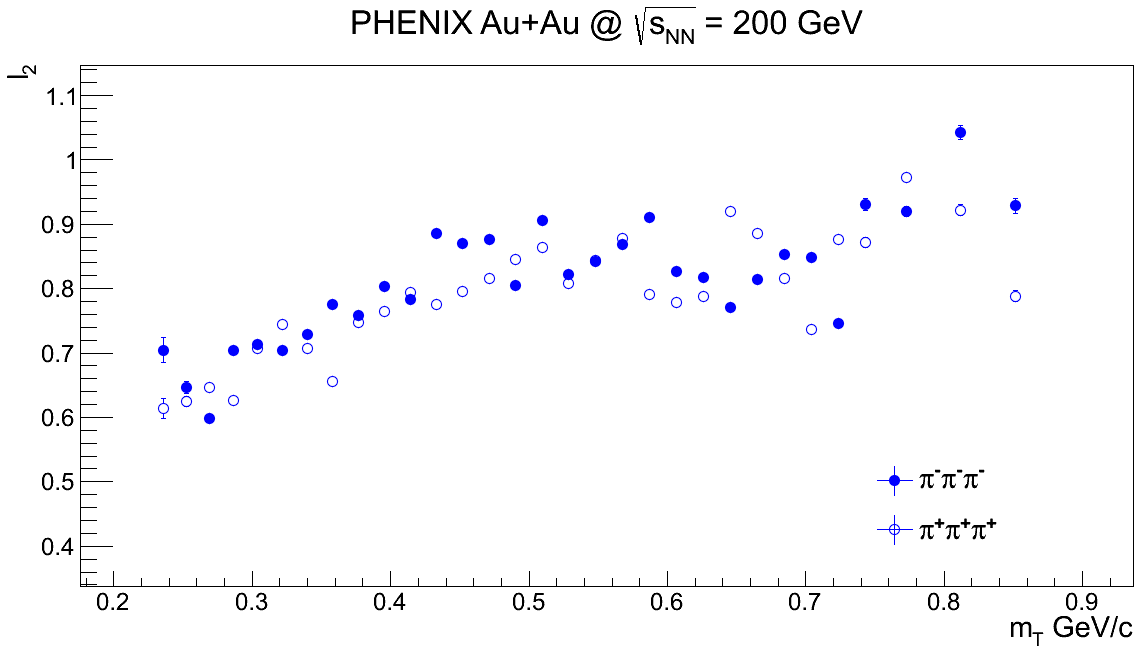
\includegraphics[scale=0.2]{pic/l2}
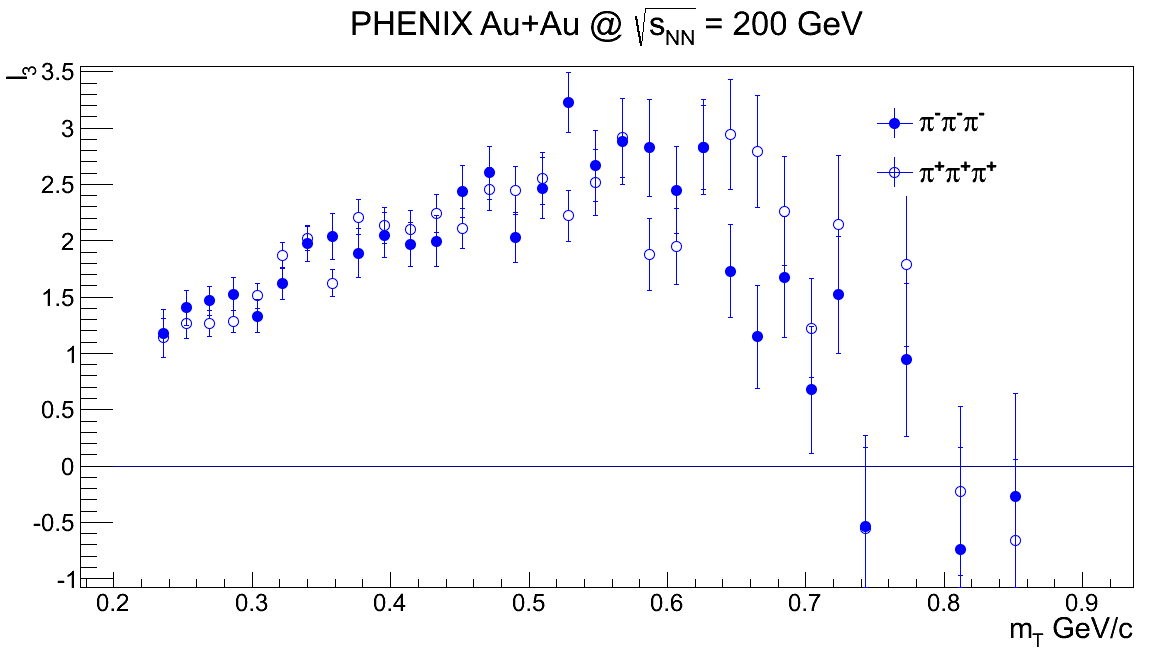
\includegraphics[scale=0.2]{pic/l3}
\end{figure}
\end{frame}


\begin{frame}
\frametitle{Derived parameter: $\lambda_3$}
\begin{itemize}
\setlength{\itemsep}{10pt}
\item Fitted: $\ell_2$, $\ell_3$, $\epsilon$, $N$; Fixed (PPG194): $R$, $\alpha$
\item $\lambda_3 := C_3(k_{12}=k_{13}=k_{23}=0)-1 = \ell_3+3\ell_2$
\item Core-Halo model: $0<\lambda_3<5$
\end{itemize}
\begin{figure}
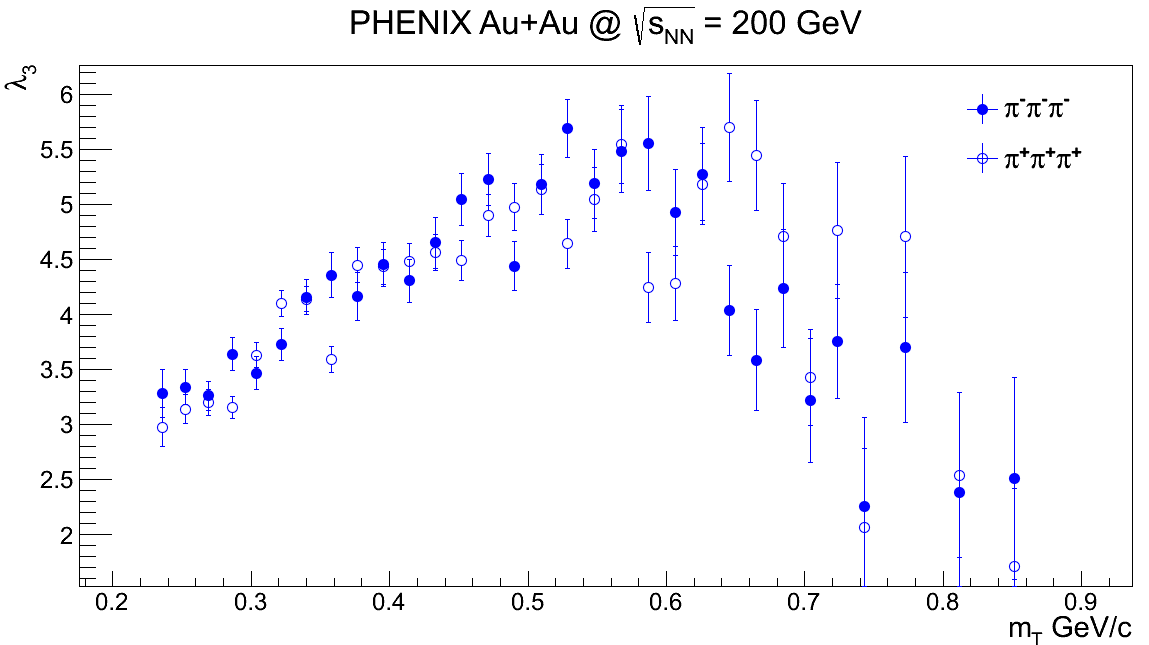
\includegraphics[scale=0.3]{pic/lambda3}
\end{figure}
\end{frame}



\begin{frame}
\frametitle{Core-Halo independent parameter}
\begin{itemize}
\item Core-Halo transformed out: $\kappa_3=\frac{\lambda_3-3\lambda_2}{2\sqrt{\lambda_2^3}}$ not depend on $f_C$ ($f_c=\mathrm{core}/(\mathrm{core}+\mathrm{halo})$)
\item This combination will be $1$ in Core-Halo
\end{itemize}
\begin{figure}
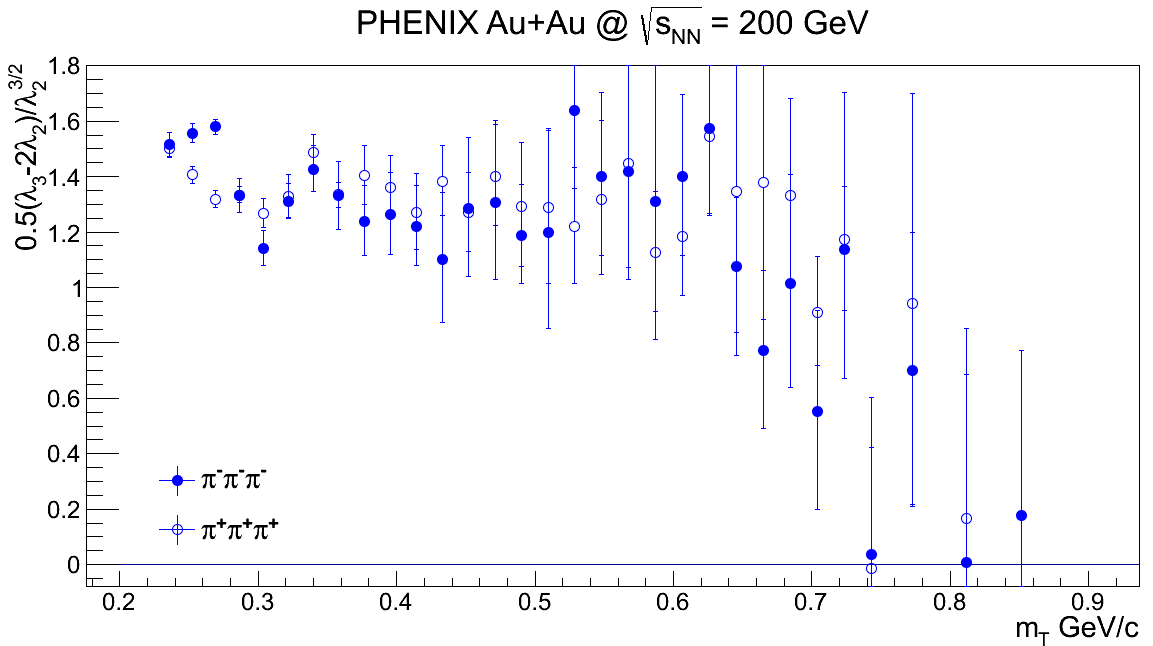
\includegraphics[scale=0.3]{pic/npar}
\end{figure}
\end{frame}


\begin{frame}
\frametitle{$f_c$ vs $p_c$}
\begin{itemize}
\item Partial coherence ($p_c=\mathrm{coherent}/(\mathrm{coherent}+\mathrm{incoherent})$, $f_c=\mathrm{core}/(\mathrm{core}+\mathrm{halo})$):

 
$\lambda_2=f_C^2\big[(1-p_c)^2+2p_c(1-p_c)\big]$
$\lambda_3=2f_C^3\big[(1-p_c)^3+3p_c(1-p_c)^2\big]+3f_C^2\big[(1-p_c)^2+2p_c(1-p_c)\big]$
\end{itemize}
\begin{figure}
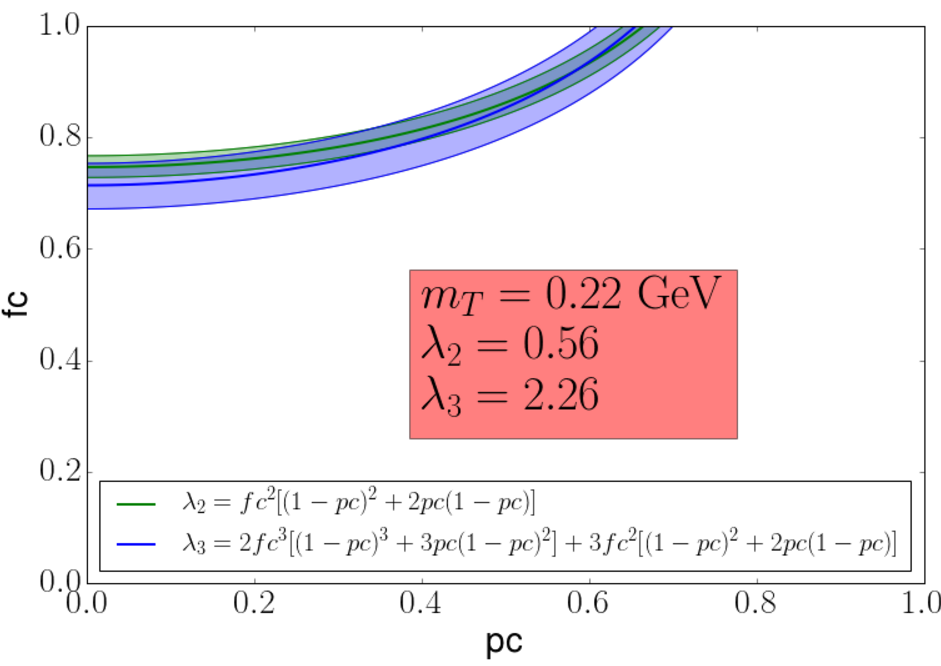
\includegraphics[scale=0.2]{pic/fcpc/5}
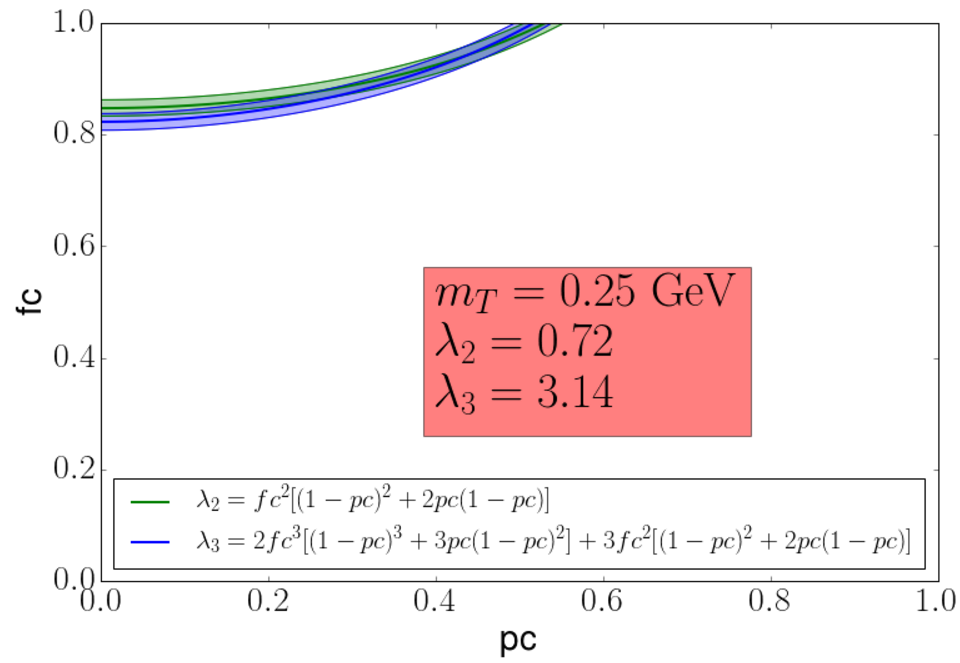
\includegraphics[scale=0.2]{pic/fcpc/9}\\
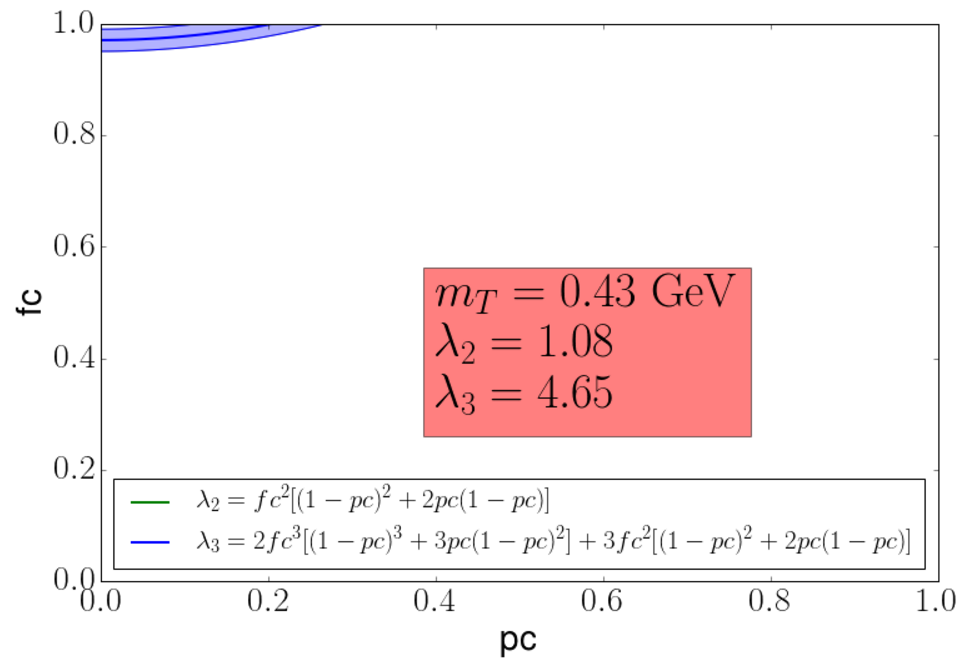
\includegraphics[scale=0.2]{pic/fcpc/3}
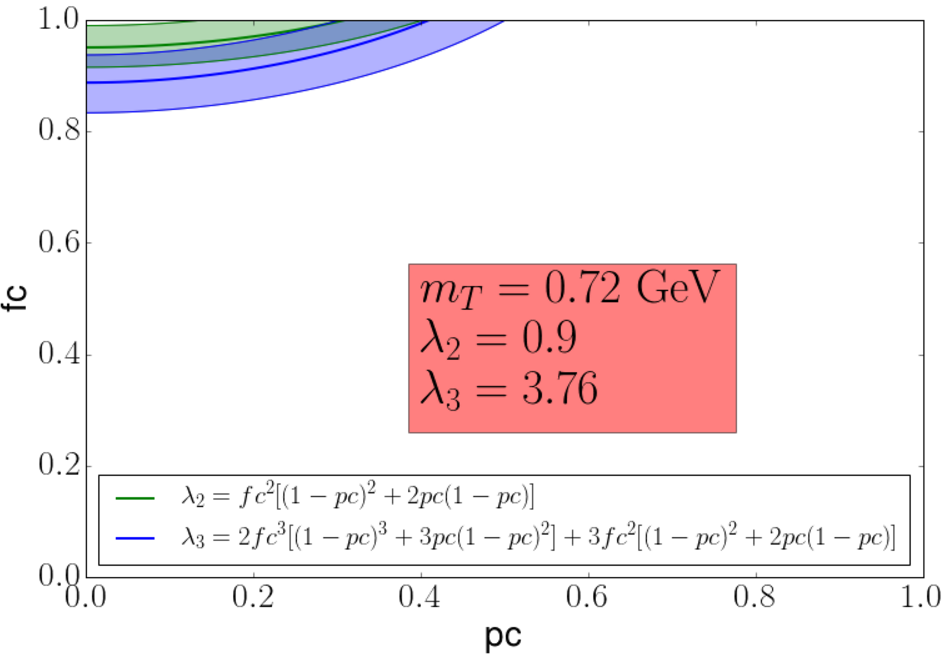
\includegraphics[scale=0.2]{pic/fcpc/4}
\end{figure}
\end{frame}


\begin{frame}
\frametitle{Consistency check: fit $\alpha$}
\begin{itemize}
\setlength{\itemsep}{10pt}
\item $\alpha$ as fitting parameter 
\item Comparing with PPG194 $\alpha$
\end{itemize}
\begin{figure}
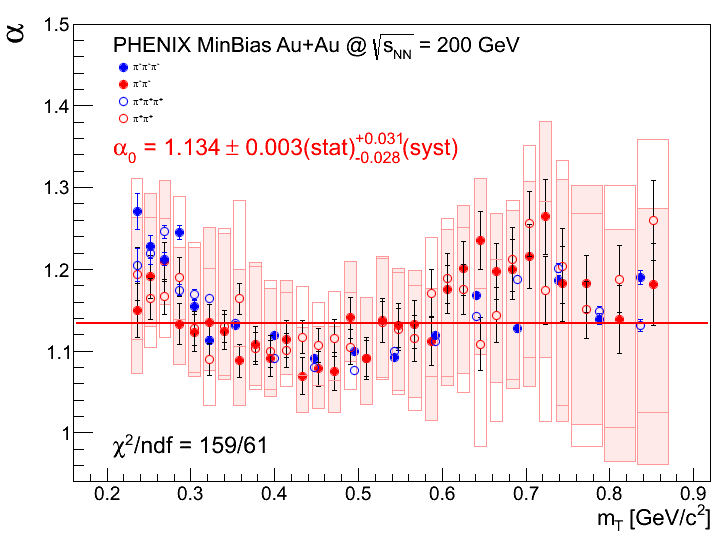
\includegraphics[scale=0.4]{pic/alpha}
\end{figure}
\end{frame}

\begin{frame}
\frametitle{Summary}
\begin{itemize}
\setlength{\itemsep}{18pt}
\item PPG194 generalized to three particle
\item Coulomb correction: Generalized Riverside
\item Good fittings: $\chi^2$ close to NDF, fitted $\alpha$ close to PPG194 $\alpha$
\item $\lambda_3$ goes above 5 (Core-Halo less then 5)
\item $\kappa_3=\frac{\lambda_3-3\lambda_2}{2\sqrt{\lambda_2^3}}$ parameter in Core-Halo 1
\item $\kappa_3$ bigger than $1$ for small $m_T$, smaller than $1$ for big $m_T$
\item We will ask preliminary for $\lambda_3$, $\kappa_3$, $f_c$ vs $p_c$
\end{itemize}

\end{frame}

\begin{frame}
\begin{center}
\Huge{Thank you for your attention!}
\end{center}
\end{frame}

\begin{frame}
\frametitle{Details of measurement}
\begin{itemize}
\setlength{\itemsep}{16pt}
\item Low bin behavior:
\begin{equation}
k_{ij}\rightarrow 0 \;\;\xRightarrow{\;\;\;?\;\;\;\;}\;\; A,B\rightarrow 0
\end{equation}
\begin{figure}
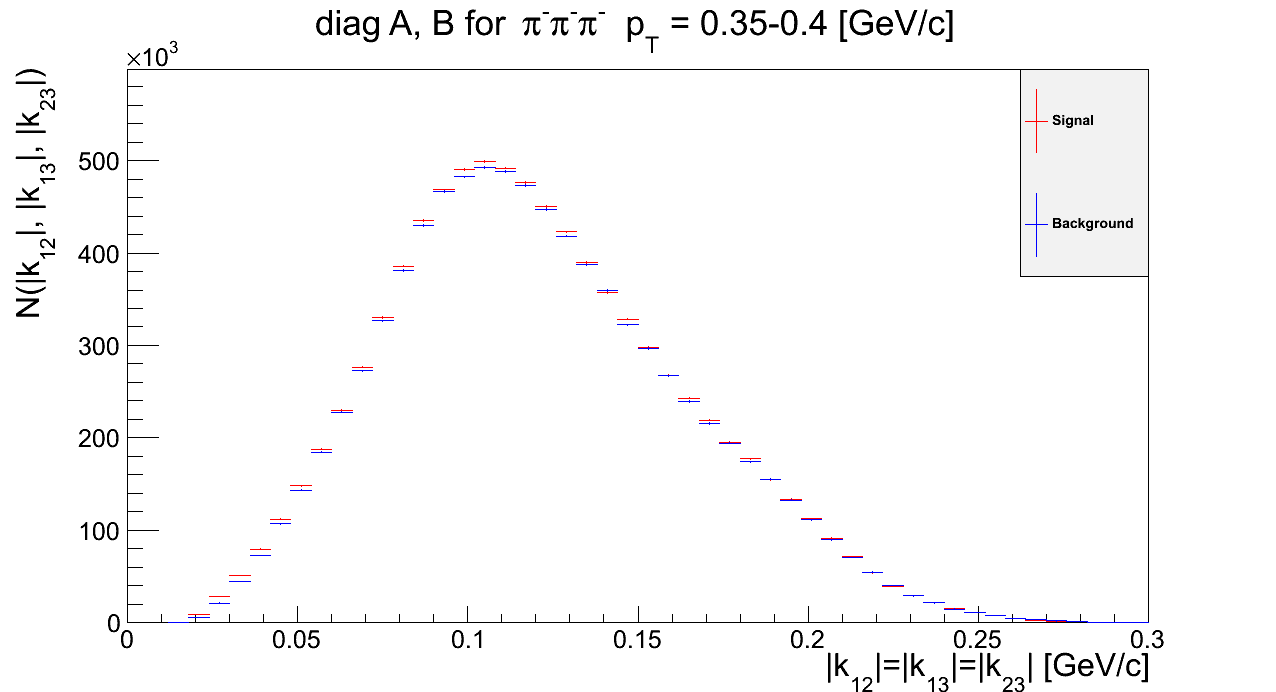
\includegraphics[scale=0.25]{pic/AB2}
\end{figure}
\end{itemize}
\end{frame}

\begin{frame}
\frametitle{Details of measurement}
\begin{itemize}
\setlength{\itemsep}{10pt}
\item The correlation:
$C_3(k_{12}, k_{13}, k_{23})=\frac{A(k_{12}, k_{13}, k_{23})}{B(k_{12}, k_{13}, k_{23})}\frac{\int B}{\int A}$
\item Triangle inequality for $\vec{k}_{12}$, $\vec{k}_{13}$, $\vec{k}_{23}$
\item Order within triplet doesn't matter
\item But when we measure do matter $\Rightarrow$ we have to fold the histogram
		$A(5,6,7) \;+=\; A(6,7,5)\; + \;A(7,5,6)\; + \;A(5,7,6)\; +...$
\end{itemize}
\begin{figure}
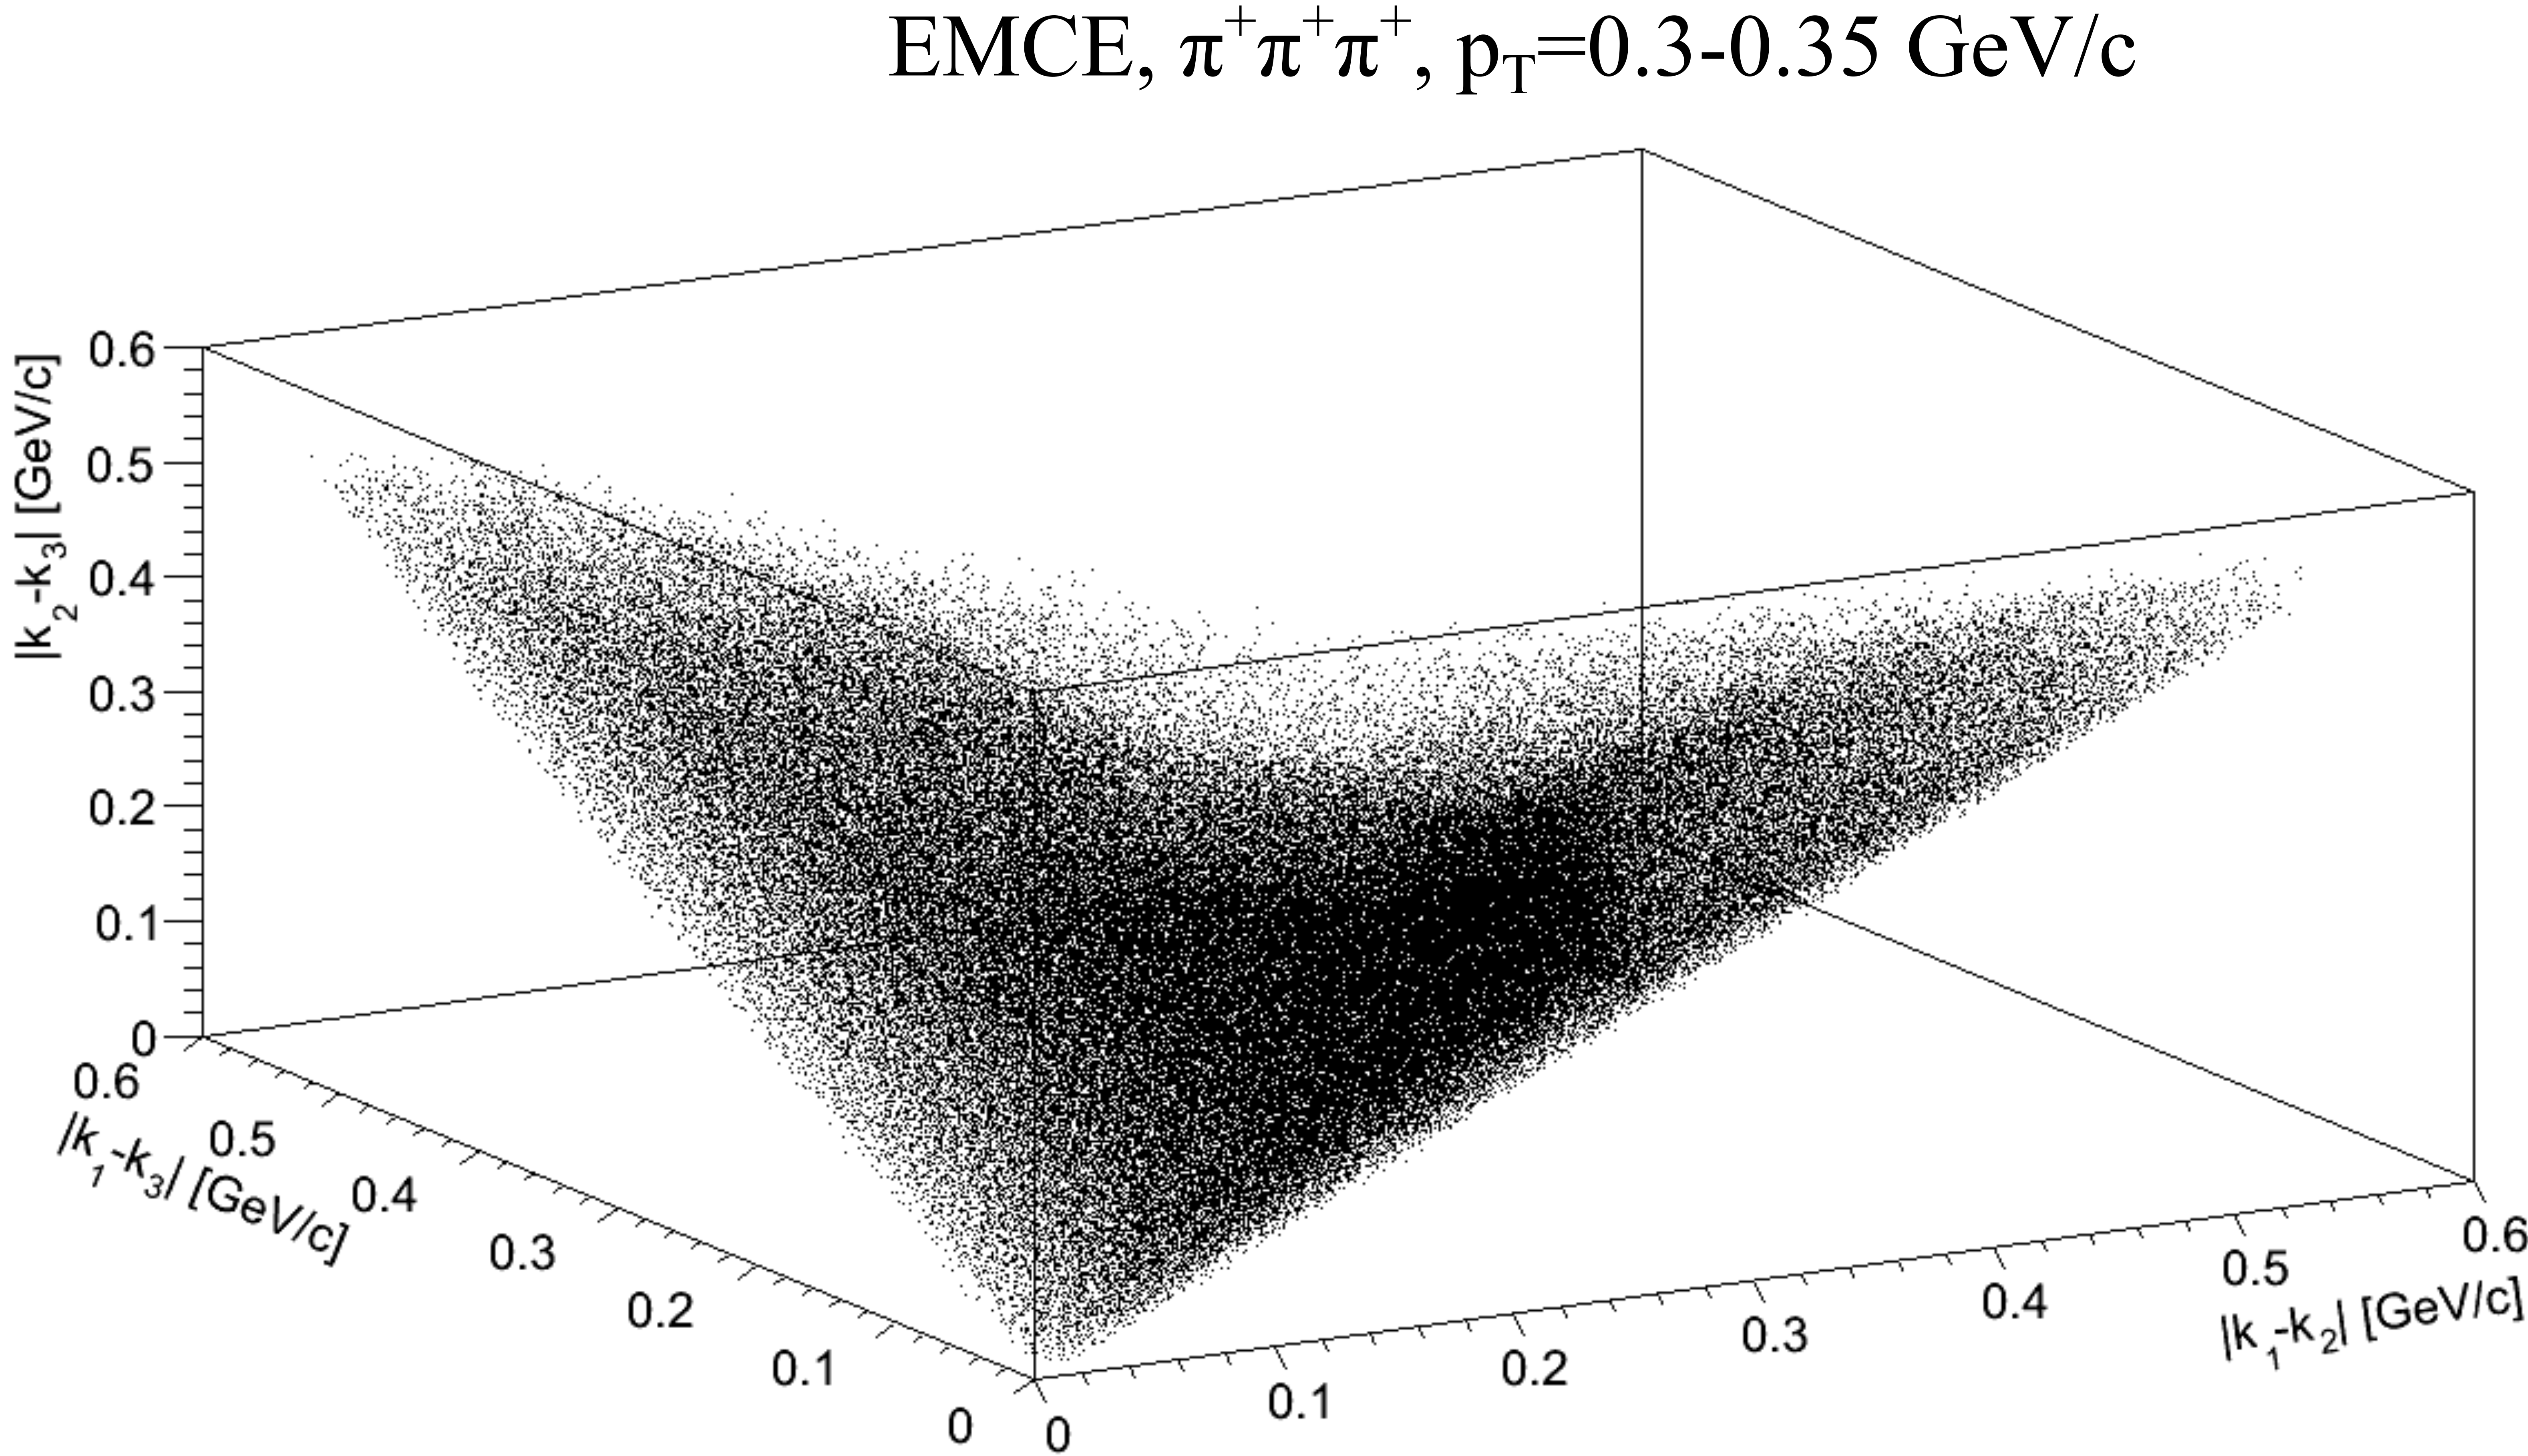
\includegraphics[scale=0.2]{pic/C1}
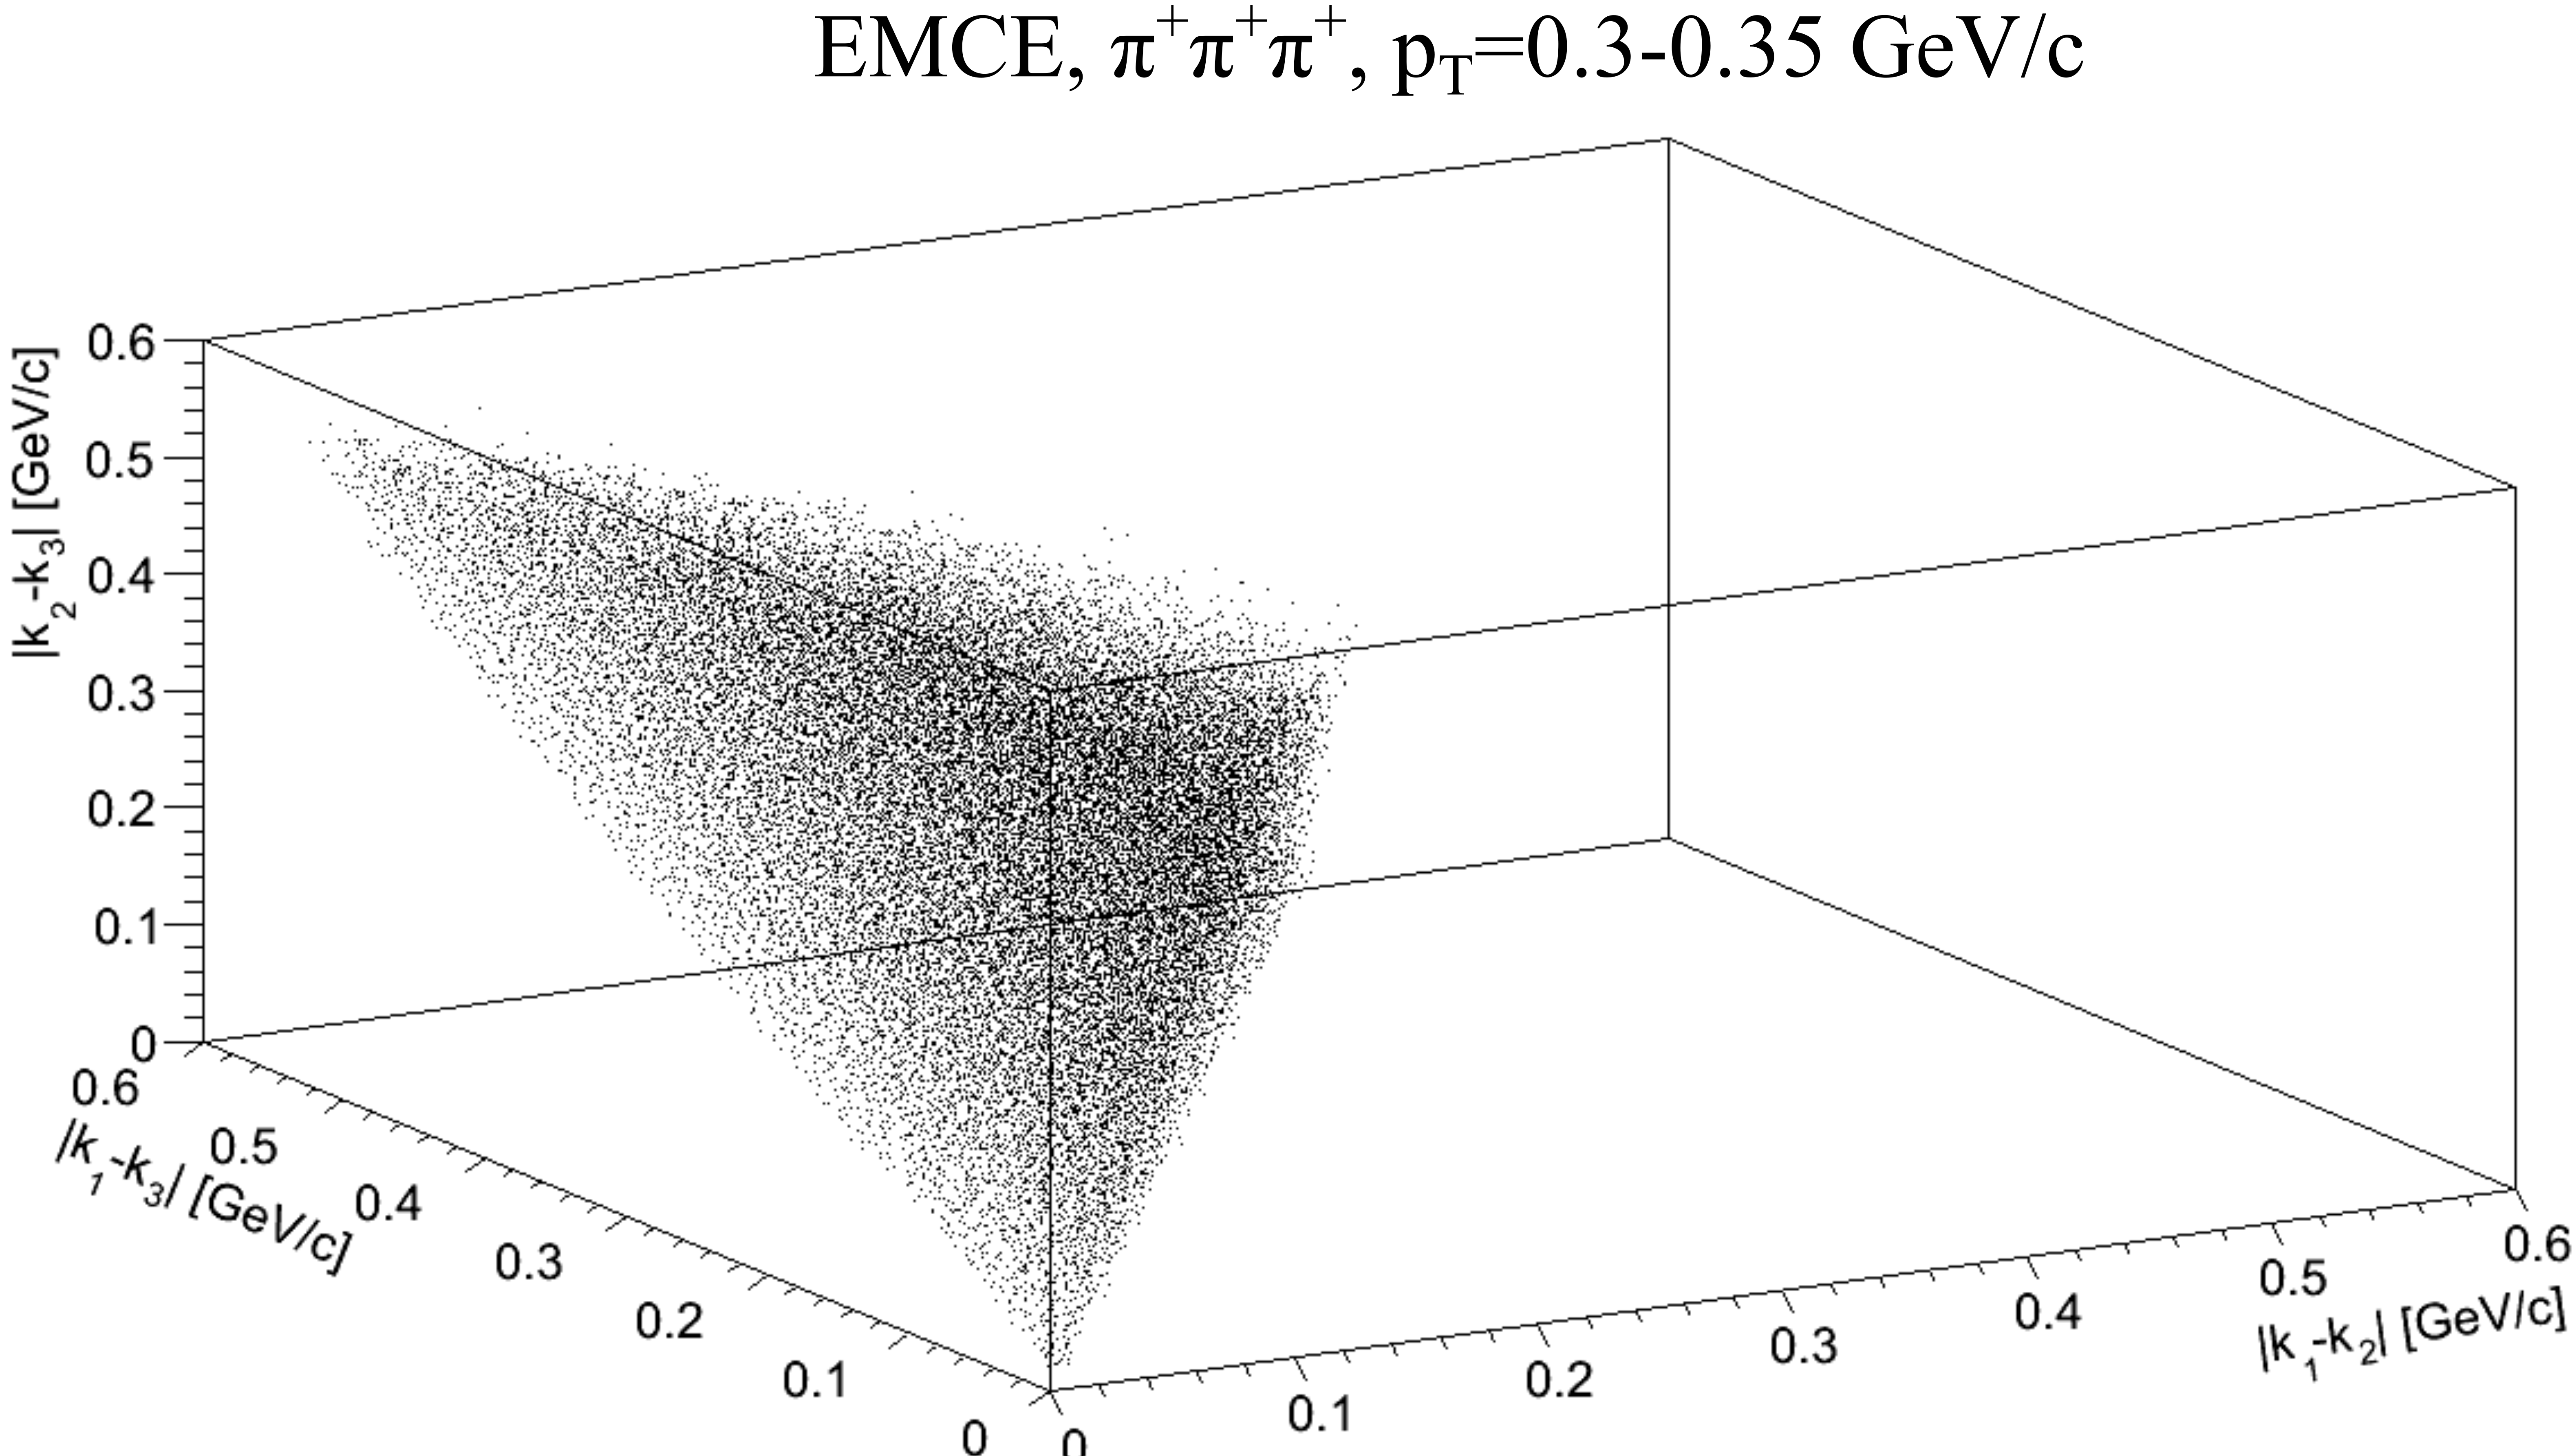
\includegraphics[scale=0.2]{pic/C2}
\end{figure}
\end{frame}

\section{Model}


\begin{frame}
\frametitle{Coulomb correction}
\begin{itemize}
\setlength{\itemsep}{16pt}
\item Corrected model:
\begin{equation}
C_3(k_{12}, k_{13}, k_{23}) = C_3^{(0)}(k_{12}, k_{13}, k_{23})\cdot K_3(k_{12}, k_{13}, k_{23})
\end{equation}
\item ''Generalized Riverside'' method for 3 particle Coulomb problem
\begin{equation}
K_3(k_{12}, k_{13}, k_{23}) \approx K_1(k_{12})K_1(k_{13})K_1(k_{23})
\end{equation}
\end{itemize}
\begin{figure}
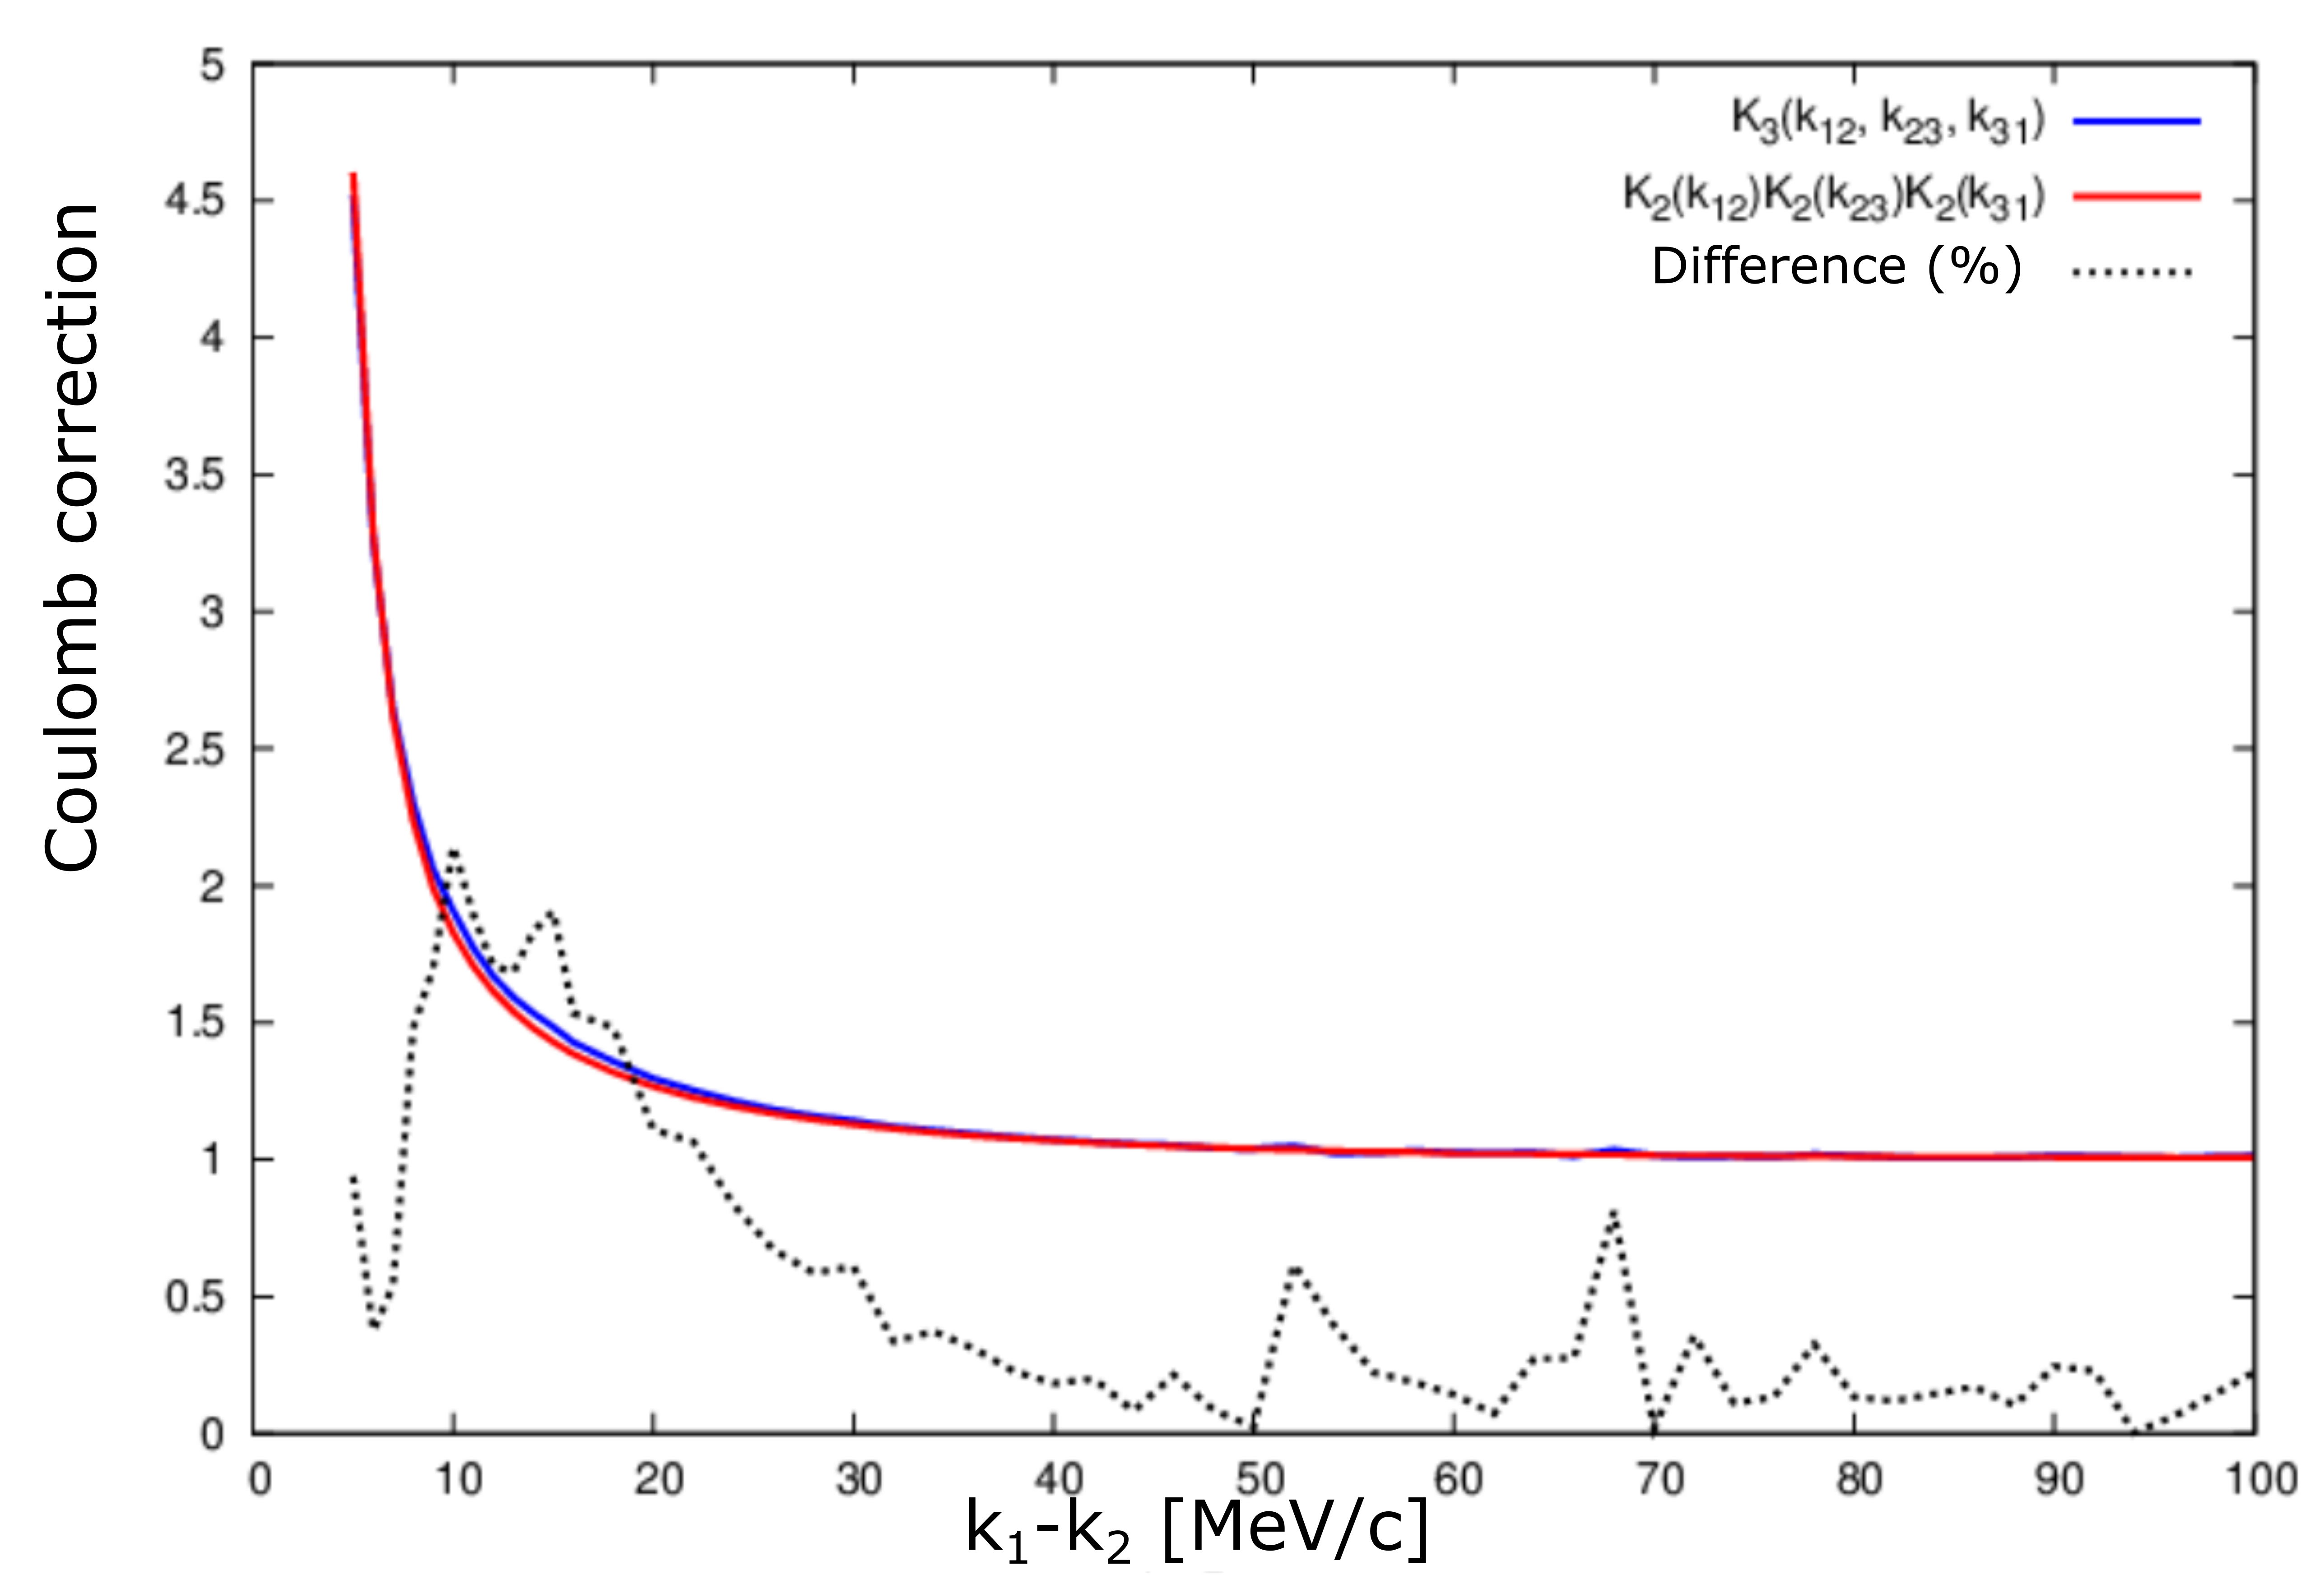
\includegraphics[scale=0.25]{pic/coulomb1}
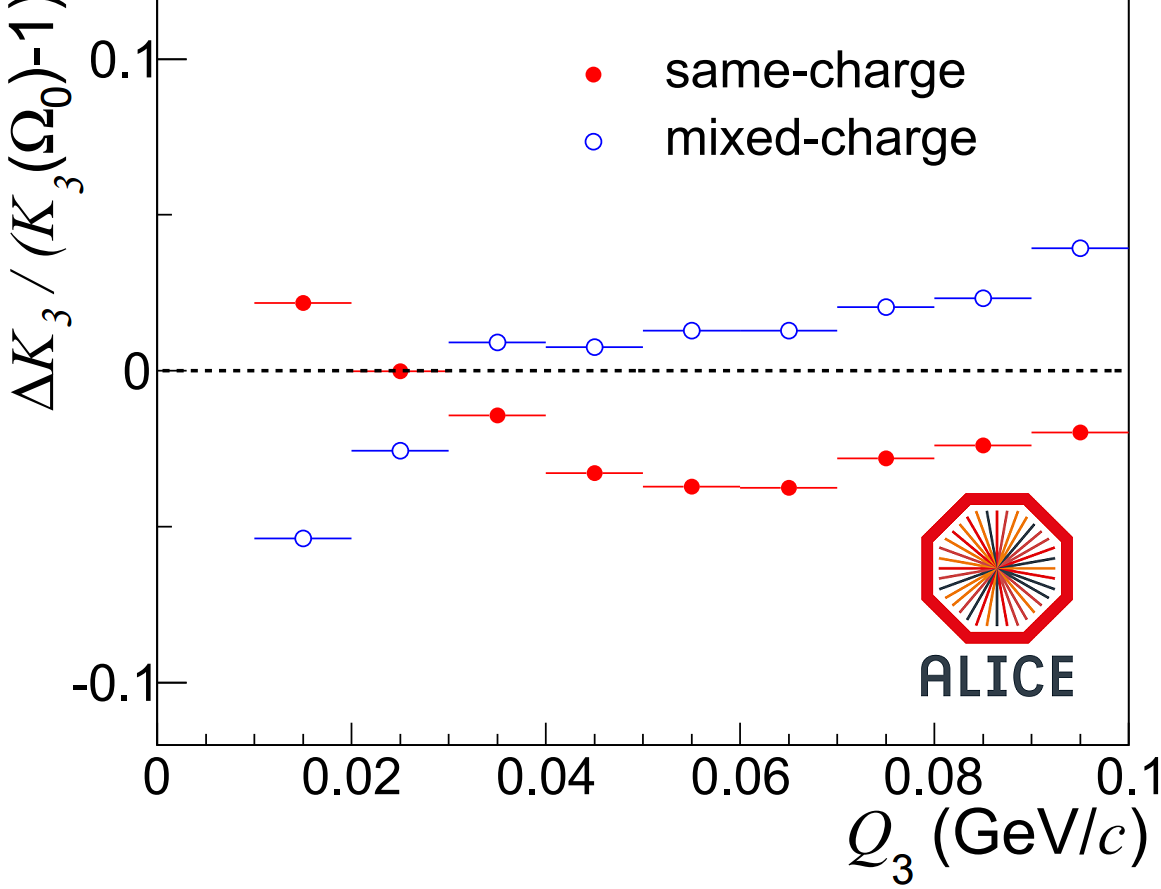
\includegraphics[scale=0.235]{pic/coulomb2}
\end{figure}
\end{frame}





\end{document}

